\documentclass[UTF8,10pt,letterpaper,fontset=none]{ctexart}

\usepackage{fontspec}
\setmainfont{TeX Gyre Termes}
\setsansfont{TeX Gyre Heros}
\setmonofont{DejaVu Sans Mono}[Scale=0.82]
\setCJKmainfont{Noto Serif CJK SC}[AutoFakeSlant=0.2]
\setCJKsansfont{Noto Sans CJK SC}
\setCJKmonofont{Noto Sans Mono CJK SC}[Scale=0.82]

\usepackage[margin=0.82in,headheight=15pt]{geometry}
\usepackage{amsmath}
\usepackage{amssymb}
\usepackage{booktabs}
\usepackage{array}
\usepackage{tabularx}
\usepackage{longtable}
\usepackage{adjustbox}
\usepackage{enumitem}
\usepackage{graphicx}
\usepackage{placeins}
\usepackage[table]{xcolor}
\usepackage[most]{tcolorbox}
\usepackage{titlesec}
\usepackage{fancyhdr}
\usepackage{siunitx}
\usepackage{tikz}
\usetikzlibrary{arrows.meta,calc,positioning}

\usepackage[
  colorlinks=true,
  linkcolor=blue!45!black,
  urlcolor=blue!55!black,
  pdftitle={紧凑型真空中极化仪探测器坐标与装配说明},
  pdfauthor={CompactInVacuum Polarimeter Project}
]{hyperref}
\usepackage{bookmark}

% --- Colors ---
\definecolor{SheetBlue}{HTML}{2E74B5}
\definecolor{SheetDark}{HTML}{1F4D78}
\definecolor{SheetMuted}{HTML}{5F6368}
\definecolor{SheetLight}{HTML}{F2F4F7}
\definecolor{SheetAmber}{HTML}{FFF4D6}
\definecolor{DetD}{HTML}{C0392B}
\definecolor{DetPL}{HTML}{2980B9}
\definecolor{DetPS}{HTML}{27AE60}

% --- Section formatting ---
\titleformat{\section}
  {\sffamily\bfseries\Large\color{SheetBlue}}
  {\thesection.}{0.55em}{}
\titleformat{\subsection}
  {\sffamily\bfseries\large\color{SheetBlue}}
  {\thesubsection}{0.55em}{}
\titlespacing*{\section}{0pt}{1.4em}{0.6em}
\titlespacing*{\subsection}{0pt}{1.0em}{0.4em}

\setlength{\parindent}{0pt}
\setlength{\parskip}{0.50em}

% --- Header/Footer ---
\pagestyle{fancy}
\fancyhf{}
\lhead{\sffamily\small\color{SheetMuted}紧凑型真空中极化仪}
\rhead{\sffamily\small\color{SheetMuted}探测器坐标与装配说明}
\cfoot{\sffamily\small\color{SheetMuted}\thepage}
\renewcommand{\headrulewidth}{0.4pt}
\renewcommand{\headrule}{\color{SheetBlue!30}\hrule width\textwidth height\headrulewidth}

\sisetup{detect-all}

% --- TikZ default node font (avoids luatexja recursion) ---
\tikzset{every node/.style={font=\sffamily\small}}

\begin{document}

% ================================================================
% TITLE
% ================================================================
\begin{center}
{\sffamily\Huge\bfseries\color{SheetBlue} 紧凑型真空中极化仪}\\[4pt]
{\sffamily\Large\color{SheetDark} 探测器坐标与装配说明}\\[2pt]
{\sffamily\normalsize\color{SheetMuted}
CompactInVacuum-afterSRC \quad\textbar\quad CompactInVacuum-preSAMURAI}\\[6pt]
{\sffamily\small\color{SheetMuted}
塑料闪烁体中心坐标表 \textbullet{} 探测器头尺寸 \textbullet{} 扇区载架装配 \textbullet{} 物理简述}
\end{center}
\vspace{0.3em}
\hrule height 1.2pt
\vspace{0.6em}

% ================================================================
\section{概述}
% ================================================================

本文件为上海谱幂（PrMat）提供紧凑型真空中极化仪（CompactInVacuum）的探测器摆放坐标与关键装配尺寸。

\begin{tcolorbox}[colback=yellow!8,colframe=orange!65!black,boxsep=4pt,left=8pt,right=8pt,top=4pt,bottom=4pt]
\sffamily\small
\textbf{状态（2026-09-01）：}本文件仅用于初步工程对接，不是加工图或采购合同。尺寸与接口以当前需求基线、resolved configuration 和验证报告为准；本文中图片仅作布局示意。
\end{tcolorbox}

极化仪采用 \textbf{d-p 弹性散射}原理测量 380\,MeV 氘核束流的张量极化度（$p_{zz}$、$p_{yy}$）。束流打在 CH$_2$ 靶上，散射的氘核和反冲质子分别由真空中塑料闪烁探测器探测，通过左右/上下对称的符合计数提取极化信息。

\textbf{核心设计参数}：

\begin{itemize}[nosep,leftmargin=1.5em]
  \item 12 个探测器（3 通道 $\times$ 4 扇区），塑料闪烁体 \varnothing 20\,mm
  \item 四扇区对称：Left（$\phi=180^\circ$）、Right（$\phi=0^\circ$）、Up（$\phi=90^\circ$）、Down（$\phi=-90^\circ$）
  \item 每扇区 1 块一体化三巢载架；afterSRC 当前仅完成初始 12\,mm 脱销/脱离支撑验证，完整取出路径待确认
\end{itemize}

\begin{tcolorbox}[colback=SheetLight,colframe=SheetBlue!40,boxsep=4pt,left=8pt,right=8pt,top=4pt,bottom=4pt]
\sffamily\small
\textbf{部署说明}：两台极化仪共用探测器头、通道坐标和三通道扇区载架的公共架构。腔体、固定支撑、检修开口、线缆终端、束流接口和完整拆装动作均按部署独立设计，不得直接复制。
\end{tcolorbox}

% ================================================================
\section{坐标系定义}\label{sec:coord}
% ================================================================

\subsection{坐标原点与轴向}

\begin{center}
\begin{tikzpicture}[scale=1.15]
  % --- z axis: horizontal RIGHT (beam direction) ---
  \draw[-{Stealth[length=5mm]},very thick,SheetBlue] (0,0) -- (4.2,0);
  \node[below,font=\sffamily\bfseries] at (4.2,-0.05) {$z$};
  \node[above,color=SheetMuted] at (2.5,0.1) {束流方向 380\,MeV d$^+$};
  % --- y axis: vertical UP ---
  \draw[-{Stealth[length=5mm]},very thick,DetPL] (0,0) -- (0,2.8);
  \node[left,font=\sffamily\bfseries,color=DetPL] at (-0.05,2.8) {$y$};
  % --- x axis: toward viewer (lower-left at ~30 deg) ---
  \draw[-{Stealth[length=5mm]},very thick,DetD] (0,0) -- (-1.6,-1.1);
  \node[below left,font=\sffamily\bfseries,color=DetD] at (-1.6,-1.1) {$x$};
  \node[below,font=\sffamily\scriptsize,color=SheetMuted] at (-0.8,-1.3) {(指向读者)};
  % --- Target at origin ---
  \fill[SheetBlue] (0,0) circle (4pt);
  \node[above right,color=SheetDark] at (0.15,0.15) {CH$_2$ 靶};
  % --- theta angle arc (from z toward y, i.e. in the y-z plane of the paper) ---
  \draw[thick,DetPS,domain=0:28] plot ({1.3*cos(\x)},{1.3*sin(\x)});
  \node[color=DetPS] at (1.3,0.28) {$\theta$};
  % --- phi angle note ---
  \node[font=\sffamily\scriptsize,color=SheetMuted,align=center] at (-3.0,2.2)
    {$\phi$: $x$--$y$ 平面\\内方位角};
  % --- Sample detector at theta~30 deg, phi=90 (in y-z plane = plane of paper) ---
  \draw[->,very thick,DetPS] (0,0) -- ({3.2*cos(30)},{3.2*sin(30)});
  \fill[DetPS] ({3.2*cos(30)},{3.2*sin(30)}) circle (5pt);
  \node[above right,color=DetPS] at ({3.2*cos(30)},{3.2*sin(30)}) {探测器};
  % --- Sector direction hints (small, in transverse plane) ---
  \node[font=\sffamily\scriptsize,color=DetPL!80] at (0.5,2.4) {Up $(\phi{=}90^\circ)$};
  \node[font=\sffamily\scriptsize,color=DetPL!80] at (0.5,-0.5) {Down $(\phi{=}{-}90^\circ)$};
  \node[font=\sffamily\scriptsize,color=DetD!80] at (-2.2,-0.6) {Right $(\phi{=}0^\circ)$};
  \node[font=\sffamily\scriptsize,color=DetD!80] at (2.3,1.5) {Left $(\phi{=}180^\circ)$};
\end{tikzpicture}
\end{center}

\subsection{球坐标约定}

\begin{itemize}[nosep,leftmargin=1.5em]
  \item 原点：CH$_2$ 靶中心，即束流轴上 $z = 0$。
  \item $\theta$（极角）：探测器方向与束流 $+z$ 轴的夹角，$0^\circ < \theta < 90^\circ$。
  \item $\phi$（方位角）：探测器方向在 $x$--$y$ 平面的投影与 $+x$ 轴的夹角。
  \item $R$（半径）：靶心到活性体中心的距离。
\end{itemize}

直角坐标换算：
\[
x = R\sin\theta\cos\phi, \quad
y = R\sin\theta\sin\phi, \quad
z = R\cos\theta
\]

% ================================================================
\section{探测器摆放坐标表}\label{sec:tables}
% ================================================================

\subsection{球坐标}

\begin{table}[h]
\centering
\sffamily\small
\caption{12 个探测器活性体中心球坐标}
\label{tab:spherical}
\renewcommand{\arraystretch}{1.25}
\begin{tabular}{ll rrr rr}
\toprule
\textbf{通道} & \textbf{扇区} & $\boldsymbol{\theta}$(°) & $\boldsymbol{\phi}$(°) & \textbf{R}(mm) & \textbf{角半宽}(°) & \textbf{立体角}(sr) \\
\midrule
\rowcolor{DetD!8}
氘核 d      & Left / Right & 20.9 & 180 / 0   & 140.0 & $\pm$4.1 & 0.0166 \\
\rowcolor{DetD!8}
            & Up / Down    & 20.9 & 90 / $-$90 & 140.0 & $\pm$4.1 & 0.0166 \\
\midrule
\rowcolor{DetPL!8}
大角质子 p$_L$ & Left / Right & 53.4 & 180 / 0   & 205.0 & $\pm$2.8 & 0.0077 \\
\rowcolor{DetPL!8}
            & Up / Down    & 53.4 & 90 / $-$90 & 205.0 & $\pm$2.8 & 0.0077 \\
\midrule
\rowcolor{DetPS!8}
小角质子 p$_S$ & Left / Right & 11.2 & 180 / 0   & 190.0 & $\pm$3.0 & 0.0089 \\
\rowcolor{DetPS!8}
            & Up / Down    & 11.2 & 90 / $-$90 & 190.0 & $\pm$3.0 & 0.0089 \\
\bottomrule
\end{tabular}
\end{table}

\subsection{直角坐标}

\begin{longtable}{ll rrr}
\caption{12 个探测器活性体中心直角坐标（mm）} \label{tab:cartesian} \\
\toprule
\sffamily\small\textbf{通道} & \sffamily\small\textbf{扇区} & \sffamily\small$\boldsymbol{x}$ & \sffamily\small$\boldsymbol{y}$ & \sffamily\small$\boldsymbol{z}$ \\
\midrule
\endfirsthead
\toprule
\sffamily\small\textbf{通道} & \sffamily\small\textbf{扇区} & \sffamily\small$\boldsymbol{x}$ & \sffamily\small$\boldsymbol{y}$ & \sffamily\small$\boldsymbol{z}$ \\
\midrule
\endhead
\rowcolor{DetD!8}
氘核 d      & Left   & $-$49.94 & $\phantom{-}$0.00 & 130.79 \\
\rowcolor{DetD!8}
氘核 d      & Right  & $\phantom{-}$49.94 & $\phantom{-}$0.00 & 130.79 \\
\rowcolor{DetD!8}
氘核 d      & Up     & $\phantom{-}$0.00 & $\phantom{-}$49.94 & 130.79 \\
\rowcolor{DetD!8}
氘核 d      & Down   & $\phantom{-}$0.00 & $-$49.94 & 130.79 \\
\midrule
\rowcolor{DetPL!8}
大角质子 p$_L$ & Left   & $-$164.58 & $\phantom{-}$0.00 & 122.23 \\
\rowcolor{DetPL!8}
大角质子 p$_L$ & Right  & $\phantom{-}$164.58 & $\phantom{-}$0.00 & 122.23 \\
\rowcolor{DetPL!8}
大角质子 p$_L$ & Up     & $\phantom{-}$0.00 & $\phantom{-}$164.58 & 122.23 \\
\rowcolor{DetPL!8}
大角质子 p$_L$ & Down   & $\phantom{-}$0.00 & $-$164.58 & 122.23 \\
\midrule
\rowcolor{DetPS!8}
小角质子 p$_S$ & Left   & $-$36.90 & $\phantom{-}$0.00 & 186.38 \\
\rowcolor{DetPS!8}
小角质子 p$_S$ & Right  & $\phantom{-}$36.90 & $\phantom{-}$0.00 & 186.38 \\
\rowcolor{DetPS!8}
小角质子 p$_S$ & Up     & $\phantom{-}$0.00 & $\phantom{-}$36.90 & 186.38 \\
\rowcolor{DetPS!8}
小角质子 p$_S$ & Down   & $\phantom{-}$0.00 & $-$36.90 & 186.38 \\
\bottomrule
\end{longtable}

\begin{tcolorbox}[colback=SheetAmber,colframe=SheetBlue!40,boxsep=3pt,left=8pt,right=8pt,top=3pt,bottom=3pt]
\sffamily\small
\textbf{注意}：上表坐标为活性体\textbf{中心}位置。活性体直径 \varnothing 20\,mm、厚度 5.5\,mm。探测器面朝靶心，即活性体前表面（面向靶的一侧）位于 $R - 2.75$\,mm 处。
\end{tcolorbox}

% ================================================================
\section{探测器头结构}\label{sec:detector}
% ================================================================

每个探测器头由以下轴向堆栈构成，总物理深度 \textbf{9.70\,mm}：
%
% \begin{center}
% \begin{tikzpicture}[scale=1.0,every node/.style={font=\sffamily\small}]
%   \def\layerH{0.55}
%   \def\layerW{3.0}
%   % Active plastic
%   \fill[DetD!30] (0,0) rectangle (\layerW,{\layerH*5.5});
%   \node[right] at ({\layerW+0.1},{\layerH*5.5/2}) {闪烁体（fast blue plastic）};
%   \node[left,color=DetD] at ({-0.1},{\layerH*5.5/2}) {5.50};
%   \pgfmathsetmacro{\ya}{\layerH*5.5}
%   % Reflector
%   \fill[DetD!15] (0,\ya) rectangle (\layerW,{\ya+0.08});
%   \node[right,font=\sffamily\scriptsize,color=SheetMuted] at ({\layerW+0.1},{\ya+0.04}) {反射层包络 0.25};
%   \pgfmathsetmacro{\yr}{\ya+0.08}
%   % Optical coupling
%   \fill[DetPS!25] (0,\yr) rectangle (\layerW,{\yr+\layerH*0.5});
%   \node[right] at ({\layerW+0.1},{\yr+\layerH*0.25}) {光耦合层};
%   \node[left,color=DetPS] at ({-0.1},{\yr+\layerH*0.25}) {0.50};
%   \pgfmathsetmacro{\yo}{\yr+\layerH*0.5}
%   % SiPM
%   \fill[DetPL!30] (0,\yo) rectangle (\layerW,{\yo+\layerH*1.5});
%   \node[right] at ({\layerW+0.1},{\yo+\layerH*0.75}) {SiPM 封装（NDL EQR15）};
%   \node[left,color=DetPL] at ({-0.1},{\yo+\layerH*0.75}) {1.50};
%   \pgfmathsetmacro{\ys}{\yo+\layerH*1.5}
%   % PCB carrier
%   \fill[gray!25] (0,\ys) rectangle (\layerW,{\ys+\layerH*1.2});
%   \node[right] at ({\layerW+0.1},{\ys+\layerH*0.6}) {传感器载板（无氧铜）};
%   \node[left,color=gray] at ({-0.1},{\ys+\layerH*0.6}) {1.20};
%   \pgfmathsetmacro{\yc}{\ys+\layerH*1.2}
%   % Rear cap
%   \fill[SheetBlue!20] (0,\yc) rectangle (\layerW,{\yc+\layerH*1.0});
%   \node[right] at ({\layerW+0.1},{\yc+\layerH*0.5}) {后安装面 / 后盖};
%   \node[left,color=SheetBlue] at ({-0.1},{\yc+\layerH*0.5}) {1.00};
%   \pgfmathsetmacro{\yend}{\yc+\layerH*1.0}
%   % Total dimension
%   \draw[<->,thick] (-1.2,0) -- (-1.2,\yend);
%   \node[left,font=\sffamily\bfseries] at (-1.3,{\yend/2}) {\rotatebox{90}{9.70 mm}};
%   % Direction arrow
%   \draw[->,thick,gray] (-0.5,-0.5) -- (1.5,-0.5);
%   \node[below,font=\sffamily\scriptsize,color=gray] at (0.5,-0.5) {面向靶（束流入射方向）};
%   \node[above,font=\sffamily\scriptsize,color=DetD] at ({\layerW/2},0.02) {$\downarrow$ 靶方向};
% \end{tikzpicture}
% \end{center}
%
% \vspace{0.3em}
\begin{center}
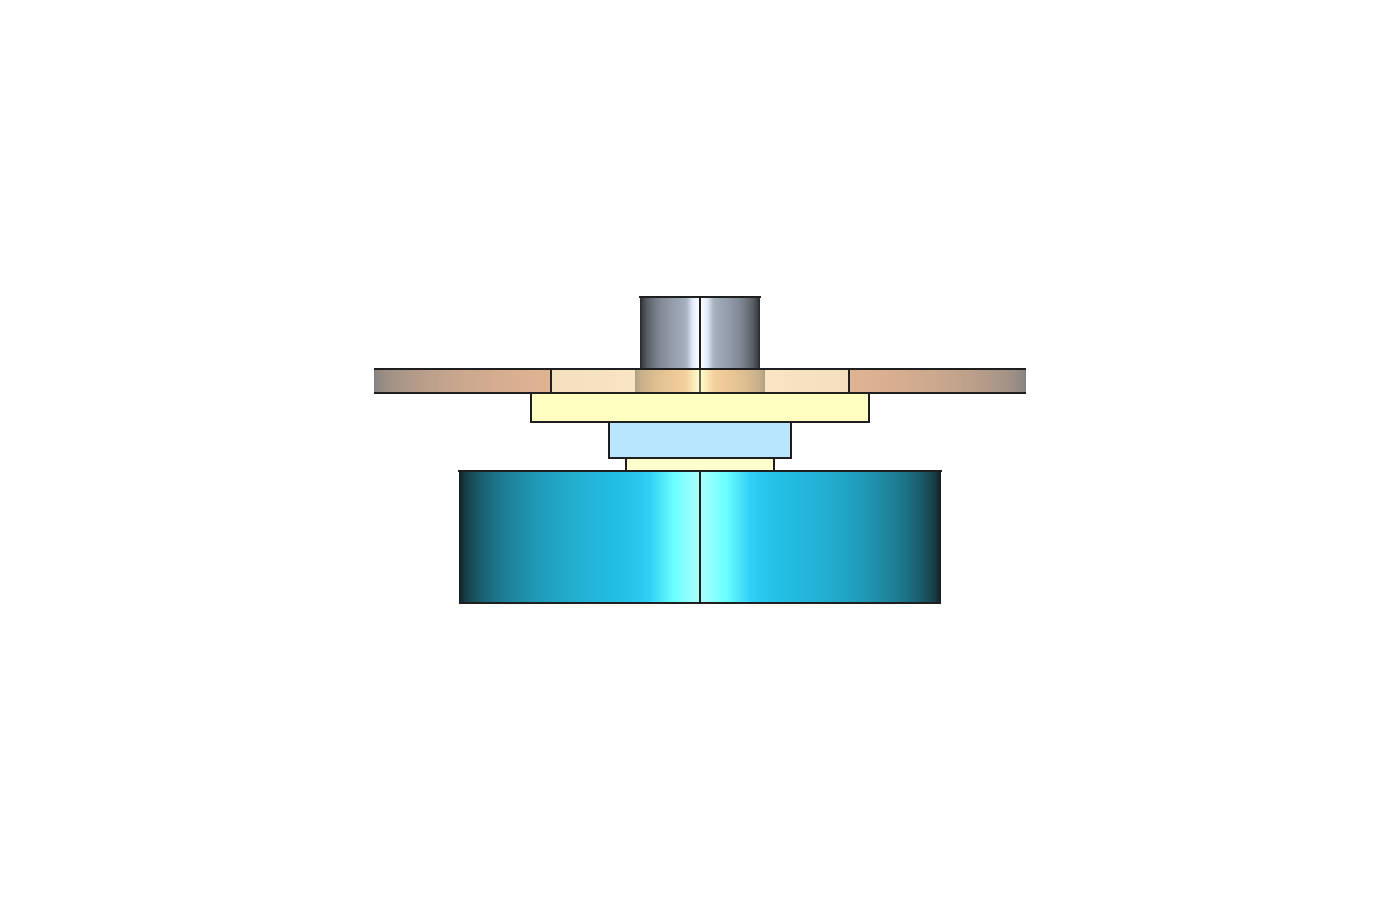
\includegraphics[width=0.62\textwidth]{figures/detector_head_transparent_side.png}
\end{center}

\begin{table}[h]
\centering
\sffamily\small
\caption{探测器头关键尺寸}
\label{tab:head}
\renewcommand{\arraystretch}{1.2}
\begin{tabular}{lr l}
\toprule
\textbf{参数} & \textbf{值} & \textbf{状态} \\
\midrule
塑料闪烁体直径        & \varnothing\,20.0\,mm & 推荐 \\
闪烁体体厚度        & 5.5\,mm & 当前 CAD 推荐原型 \\
外壳外径          & \varnothing\,23.0\,mm & — \\
SiPM 候选        & NDL EQR15 11-6060D-S & 推荐 \\
\bottomrule
\end{tabular}
\end{table}

% ================================================================
\section{扇区载架与四扇区总装}\label{sec:assembly}
% ================================================================

\subsection{单扇区载架}

每个扇区由\textbf{一块整体载板}承载三个探测器头（氘核 + 大角质子 + 小角质子）。载板上加工有：
\begin{itemize}[nosep,leftmargin=1.5em]
  \item 3 个圆柱形巢座（含 D 型平面防转特征）
  \item 3 个可拆卸压桥（M3 紧固件）
  \item 3 个接收窗（避开粒子飞行路径）
  \item 1 个平面--销--槽腔体接口
  \item 1 条后部公共走线槽
\end{itemize}

维护方式：松开压桥 $\to$ 探测器沿轴向后方取出。afterSRC 扇区载架在固定腔壁支撑上完成平面--销--槽定位；当前实体位姿只验证向腔内移动 12\,mm 以脱开定位销的初始释放阶段。后续平移、转姿并通过顶部 ICF305 孔径提出的连续动作仍待 STEP 验证；旧 70\,mm 直线径向路径不是完整取出证据。

\begin{center}
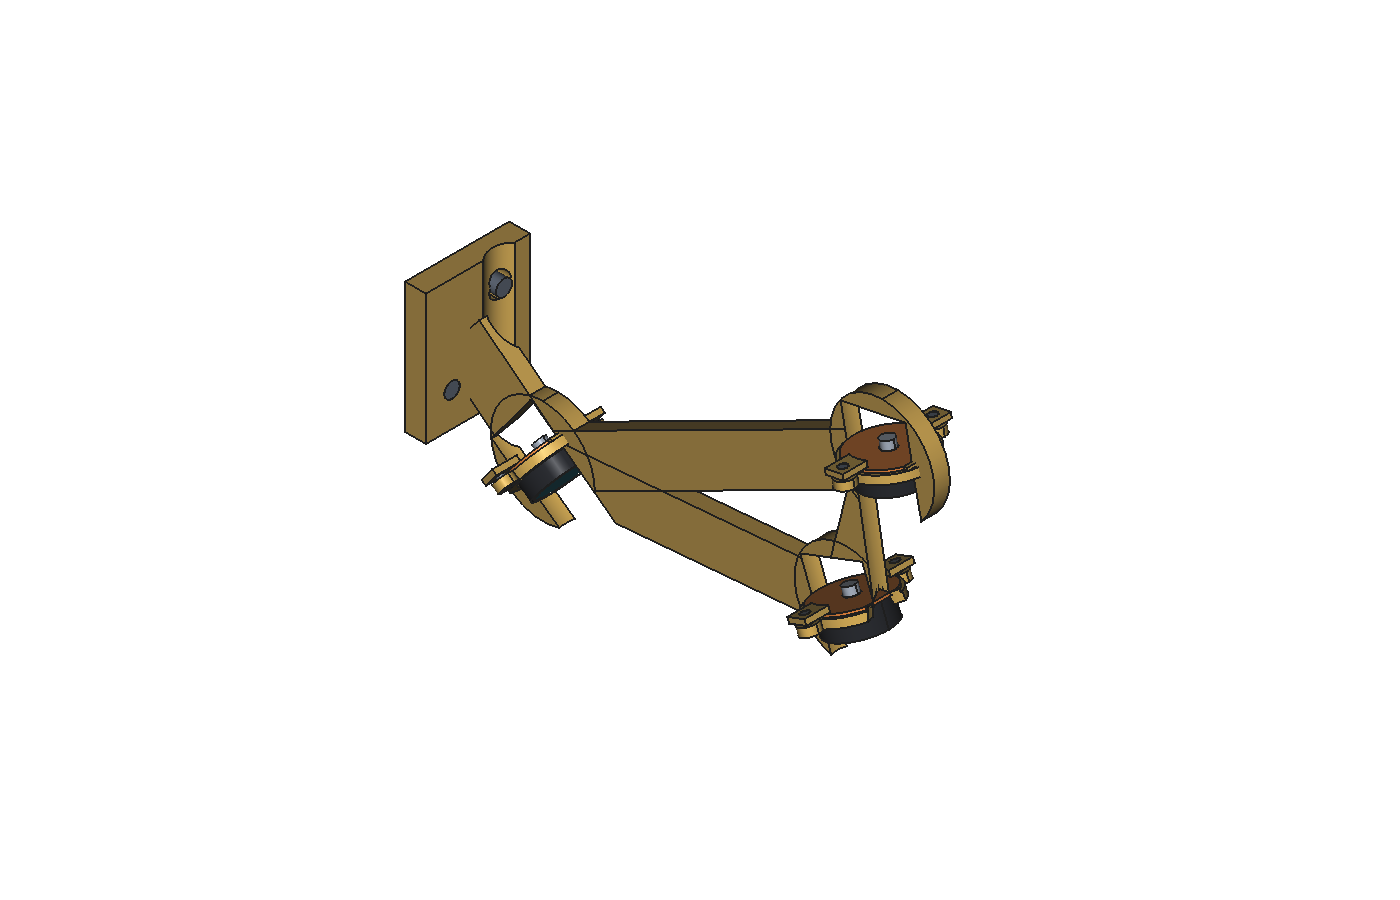
\includegraphics[width=0.58\textwidth]{figures/sector_holder_isometric.png}
\end{center}

\begin{tcolorbox}[colback=SheetLight,colframe=SheetBlue!30,boxsep=3pt,left=7pt,right=7pt,top=3pt,bottom=3pt]
\sffamily\scriptsize\color{SheetMuted}
不再在公共坐标表中使用 2026-08-03 的四向对称支撑截图。该图早于 afterSRC ICF305 固定墙支撑改造，会误导顶部支撑归属。单扇区载架是公共架构；四扇区在腔体内的支撑、定位和取出方式按部署独立评审。
\end{tcolorbox}

\subsection{四扇区总装与靶位置}

四个扇区载架以 90$^\circ$ 间隔安装在真空腔内。靶机构为旋转式，靶片在 work 状态位于坐标原点，在 park 状态转至腔壁附近。当前 ICF70 只是旋转馈通的工程研究包络，最终法兰和购买件需分部署确认。

\begin{table}[h]
\centering
\sffamily\small
\caption{靶位置}
\label{tab:target}
\renewcommand{\arraystretch}{1.2}
\begin{tabular}{lrrr l}
\toprule
\textbf{状态} & \textbf{x}(mm) & \textbf{y}(mm) & \textbf{z}(mm) & \textbf{角度} \\
\midrule
Work（测量）  & 0 & 0 & 0 & 0$^\circ$ \\
Park（移开）  & 70 & 0 & 70 & 90$^\circ$ \\
\bottomrule
\end{tabular}
\end{table}

% ================================================================
\section{物理简述}\label{sec:physics}
% ================================================================

\subsection{测量原理}

极化仪利用 \textbf{H(d,d)p 弹性散射} 测量 380\,MeV 氘核束流的张量极化度 $p_{zz}$ 和 $p_{yy}$。极化氘核打在 CH$_2$ 靶上，散射氘核与反冲质子由方位角相差 180$^\circ$ 的探测器对符合测量。

在给定氘核实验室角 $\theta_d$，弹性散射有两个质心分支（前向 / 后向），对应两个不同能量的氘核和两个不同角度的反冲质子：

\begin{table}[h]
\centering
\sffamily\small
\caption{符合分支配置（380\,MeV d-p 弹性）}
\label{tab:branches}
\renewcommand{\arraystretch}{1.25}
\begin{tabular}{ll ccc l}
\toprule
\textbf{分支} & \textbf{用途} & $\boldsymbol{\theta_d}$(°) & \textbf{质子探测器} & $\boldsymbol{\theta_p}$(°) & \textbf{T20} \\
\midrule
\rowcolor{SheetLight}
前向 (forward) & $p_{zz}$ 分子、$p_{yy}$ & 20.9 & p$_L$ & 53.4 & $+$0.151 \\
\rowcolor{SheetAmber!50}
后向 (backward) & $p_{zz}$ 分母 & 20.9 & p$_S$ & $\sim$10.9$^\dagger$ & $-$0.350 \\
\bottomrule
\end{tabular}
\end{table}

\noindent\textsuperscript{$\dagger$}\,后向分支反冲质子运动学中心约 10.9$^\circ$，p$_S$ 探测器置于 11.2$^\circ$，其 $\pm$3$^\circ$ 角接收范围完全覆盖。氘核探测器角半宽 $\pm$4.1$^\circ$，后向质子覆盖范围 8$^\circ$--14.5$^\circ$，与 p$_S$ 接收范围（8.2$^\circ$--14.2$^\circ$）高度重叠。

\subsection{符合对配置}

共 8 组符合对（2 分支 $\times$ 4 扇区），每对中氘核与质子在方位角上严格相差 180$^\circ$：

\begin{table}[h]
\centering
\sffamily\small
\caption{8 组符合对（每支 4 对）}
\label{tab:coincidence}
\renewcommand{\arraystretch}{1.15}
\begin{tabular}{lll rr}
\toprule
\textbf{分支} & \textbf{氘核探测器} & \textbf{配对质子探测器} & \textbf{方位角差} & \textbf{极限立体角}(sr) \\
\midrule
前向 & Left d  & Right p$_L$  & 180$^\circ$ & 0.0077 \\
前向 & Right d & Left p$_L$   & 180$^\circ$ & 0.0077 \\
前向 & Up d    & Down p$_L$   & 180$^\circ$ & 0.0077 \\
前向 & Down d  & Up p$_L$     & 180$^\circ$ & 0.0077 \\
\midrule
后向 & Left d  & Right p$_S$  & 180$^\circ$ & 0.0089 \\
后向 & Right d & Left p$_S$   & 180$^\circ$ & 0.0089 \\
后向 & Up d    & Down p$_S$   & 180$^\circ$ & 0.0089 \\
后向 & Down d  & Up p$_S$     & 180$^\circ$ & 0.0089 \\
\bottomrule
\end{tabular}
\end{table}

$p_{zz}$ 的测量公式为前后分支符合计数比：
\[
R = \frac{N_\text{前向}}{N_\text{后向}}, \qquad
p_{zz} \propto \frac{R - R_0}{\Delta T_{20}}
\]
其中 $R_0$ 为未极化时的比值，$\Delta T_{20}$ 为前后分支张量分析本领之差。后向分支 $|T_{20}| = 0.350$（相对不确定度 $\sim$3.4\%）优于前向 $|T_{20}| = 0.151$（$\sim$10.6\%），是 p$_{zz}$ 测量的关键通道。

% ================================================================
\section{两个部署的腔体对比}\label{sec:deploy}
% ================================================================

两台极化仪共用探测器坐标和扇区载架概念；腔体、固定支撑、检修动作和所有外部接口分别关闭：

\begin{table}[h]
\centering
\sffamily\small
\caption{两个部署的腔体与接口对比}
\label{tab:deploy}
\renewcommand{\arraystretch}{1.3}
\begin{tabularx}{\textwidth}{l X X}
\toprule
 & \textbf{afterSRC} & \textbf{pre-SAMURAI} \\
\midrule
安装位置      & SRC 下游 & SAMURAI 终端上游 \\
腔体截面      & 方形 440 $\times$ 440\,mm & 方形 450 $\times$ 450\,mm \\
腔体长度      & 420\,mm（内净 404\,mm） & 380\,mm（内净 364\,mm） \\
壁厚          & 8\,mm（provisional） & 8\,mm（provisional） \\
材料          & 304L 不锈钢 & 304L 不锈钢 \\
前端接口      & ICF114 布置包络，站点 TBD & VF100 继承包络，站点 TBD \\
后端接口      & ICF114 布置包络，站点 TBD & VG80 继承包络，站点 TBD \\
顶部检修口    & ICF305 全金属盲板（推荐原型） & TBD \\
靶馈通        & ICF70 研究包络，站点 TBD & 站点 TBD \\
信号馈通      & 4 $\times$ ICF70 容量研究，站点 TBD & 4 $\times$ ICF70 容量研究，站点 TBD \\
束流通径      & 站点 TBD（当前 CAD 过渡管内径 \varnothing\,60.2\,mm） & 站点 TBD（当前包络 \varnothing\,80\,mm） \\
扇区支撑      & 固定腔壁支撑；检修盲板不承载 & 按站点独立设计 \\
\bottomrule
\end{tabularx}
\end{table}

\begin{tcolorbox}[colback=white,colframe=SheetBlue!35,boxsep=4pt,left=8pt,right=8pt,top=4pt,bottom=4pt]
\sffamily\small
\textbf{CAD 图片状态：}旧 360\,mm/顶部服务口截图已从本表撤下，避免将旧支架位置误读为当前结构。评审时应打开 canonical \texttt{CompactOne\_afterSRC.FCStd/STEP}，确认 ICF305 盲板不承载内部支架，并分别检查固定支撑和完整取出动作。
\end{tcolorbox}

\begin{tcolorbox}[colback=SheetLight,colframe=SheetBlue!30,boxsep=4pt,left=8pt,right=8pt,top=4pt,bottom=4pt]
\sffamily\small\color{SheetMuted}
\textbf{关于 provisional 标注}：上述壁厚、束流接口、旋转/信号馈通和 ICF305 购买件尺寸均需由批准的现场测量、购买件认证图纸、外压结构计算和完整拆装验证关闭后方可用于加工制造。afterSRC 顶部盲板只封闭真空边界，不作为探测器支架或定位基准。
\end{tcolorbox}

% \vspace{1em}
% \hrule height 0.5pt
% \vspace{0.3em}
% {\sffamily\scriptsize\color{SheetMuted}
% 本文档坐标数据来源于 \texttt{compactInVacuum/config/common\_detector.yaml} 和 FreeCAD 验证报告。物理分析本领数据来源于 Sekiguchi et al.\ 的 d-p 弹性散射实验测量。}
%
\end{document}
